\chapter{СУЧАСНИЙ ПОГЛЯД НА ДІАГНОСТИКУ ТА ЛІКУВАННЯ ГЕПАТОБЛАСТОМ У ДІТЕЙ (огляд літератури)}

\section{Вступ}
Пухлини печінки у дітей охоплюють широкий спектр новоутворень, починаючи від доброякісних до злоякісних. Кожне з новоутворення має cвої особливості та різні  прогнози. Гепатобластома є найбільш поширеною пухлиною печінки дитячого віку. Найбільш вагоме покращення результатів лікування гепатобластоми відбулося з моменту початку використання хіміотерапії наприкінці 1970-х років. 

У період «темних віків» протягом багатьох століть, діти не вважалися частиною суспільства, їхньому становищу приділялося мало уваги, а особливо їхнім захворюванням. Тому не дивно, що важко знайти будь-яку інформацію на рахунок даного питання у медичній літературі. Пухлини будь-якого органу, включаючи печінку, були зафіксовані як хвороби, пов'язані з усіма видами містичних або релігійних причин, з відповідним лікуванням. Хірургія була сферою навчання хірургів, які виконували "примітивні" хірургічні операції, скоріше як видовище для глядачів. У XIX столітті з’явились перші дитячі відділення та лікарні

Одним із перших сучасних лікарів, який присвятив себе написанню монографії про дитячі пухлини, був Вілліс \cite{pmid10466608}. Він чітко розрізнив ембріональний тип та карциному. 
Методи хірургічного втручання на печінці суттєво не відрізняються у дорослих та дітей, а оскільки захворювання у дорослих зустрічаються набагато частіше, не дивно, що “дорослі” хірурги взяли на себе ініціативу в цих розробках. 

В одній із перших ранніх згадок про резекції печінки у дітей була представлена серія із 19 випадків пухлин у дітей, 14 із яких були злоякісні пухлини,  із яких вижили лише 3 дитини. Інтраопераційна смертність від кровотечі склала 3\%. Однак у іншому спостереженні \cite{pmid10839879} із 11 резекцій (6 з гепатобластомою) у дітей у віці від 7 днів до 14 років не було інтраопераційної летальності, окрім одного летального випадку через 8 місяців після операції. 

Основними причинами високої захворюваності та смертності при резекціях печінки були кровотечі та біліарні ускладення, що виникали через погане розуміння сегментарної судинної та жовчної анатомії печінки, яку описав Куіно в 1954 р. \cite{pmid12778356}. У цей період опублікувано результати дослідежння з летальністю після резекцій печінки понад 10\%. Для зменшення інтраопераційної крововтрати рутинно почали використано різні пройоми, наприклад, прийом Pringle \cite{pmid15285242} (затискання печінкової судинної ніжки); тотальна оклюзія судин (затискання аорти та балонна оклюзія нижньої порожнистої вени з  переохолодженням \cite{pmid1328586}; передрезекційна перев'язка ворітної вени, печінкової артерії та/або печінкових вен; гіпотензивна анестезія. Були розроблені різні методики транссекції паренхіми печінки для зменшення крововтрати, наприклад ультразвуковий дисектор – CUSA. 

Однак, в основному, покращення результатів резекцій печінки було пов’язано з вивченням та широким впровадженням в хірургічну практику внтрішньопечінкової класифікації сегментів Куіно, які зараз є загальновизнаними як золотий стандарт у хірургії печінки \cite{pmid12778356}. До цього термінологія резекцій печінки була заплутаною та неправильною, та спиралась на анатомію правої, лівої частках та умбілікальної борозни, яка не відповідає судинному постачанню та жовчній архітектектоніці.
В останні роки смертність та захворюваність у спеціалізованих печінкових центрах нижче 5\%. 

Трансплантація печінки та інших органів стала можливою після досліджень про відторгнення та його запобігання за допомогою імуносупресій. Цей метод лікування все частіше почали використовувати при лікування гепатобластом. Для більш широкого впровадження трансплантації печінки у дітей залишається не вирішеними питання нехватки органів та необхідна пожиттєва імуносупресія. Недостача донорських органів вирішують впровадженням живого родинного донорства та розділенням цілої печінки при трупній трансплантації \cite{pmid14746860}. 

\section{Епідеміологія та онкологічні аспекти гепатобластом}
Новоутворення печінки у дітей раннього віку часто є злоякісними, при цьому гепатобластома є найпоширенішим первинним дитячим злоякісним новоутворенням  печінки. Захворюваність гепатобластомою становить 1,2–1,5 на мільйон людей на рік. Більшість гепатобластом  діагностуються у дітей старше 3 років, в той час, як у дітей старше  4 років дане захворювання є вкрай рідкісним. Більшість випадків гепатоблстоми носять спорадичний характер, не маючи відомих на те причин, до встановлених факторів ризику відносять недоношеність і низьку вагу при народженні, а також сімейний аденоматозний поліпоз, синдром Беквіта-Відемана та трисомію 18 хромосоми \cite{pmid15285242}. 

Щодо факторів зовнішнього середовища є дані про підвищений ризик появи гепатобластоми у дітей, матері яких палять, а також у дітей, батьки яких обоє палять. 

Статистично достовірний зв'язок гепатобластоми та низької маси тіла при народженні вперше було виявлено групою японських авторів \cite{pmid14752798} та неодноразово підтверджено іншими авторами \cite{pmid14746860}. Було встановлено підвищений рівень захворюваності у дітей з масою тіла при народженні менше 1500 г, і ще більше при масі тіла менше 1000г \cite{pmid15285242}.
У випадках НВ повідомляється про широкий спектр синдромів вроджених вад розвитку та ізольованих аномалій. Загальна частота аномалій серед дітей з НВ є вищою, ніж для будь-якої дитячої пухлини, 
крім Вільмса \cite{pmid15285242}. Повідомлення про випадки включають дітей із прогресуючим сімейним холестазом, мієлодисплазією, синдромом Нунана, синдромом Тендітного Х, синдромом Сотоса, синдромом Кардіо-Фаціо, Синдромом Прадера-Віллі, Голденхаром та нейрофіброматозом типу 1 \cite{pmid25649007}.

Етіологічне значення цих різних синдромів є невизначеним, але слід враховувати можливі зв’язки з недоношеними/низькою вагою при народженні та доглядом за новонародженими, а також генетичні зв’язки.
На додаток до випадкових повідомлень про випадки НВ у синдромних дітей, було встановлено три стани, що призводять до підвищеного ризику НВ: трисомія 18, синдром Беквіта-Відемана (BWS) та сімейний аденоматозний поліпоз (FAP). Трисомія 18 або синдром Едвардса (ES) пов'язані з множинними вродженими аномаліями, включаючи вади серця, черепно-лицьові аномалії, аномалії кінцівок та інших скелетів, мікроцефалію, затримку розумового розвитку, затримку внутрішньоутробного розвитку та низький зріст. 
Повідомляється про частоту розвитку ЕС на 1 з 3000 до 7000 народжень. Виживання після першого року рідкісне \cite{pmid14966740}. Зараз зафіксовано щонайменше сім випадків НВ у дітей із ES. Це свідчить про етіологічний зв’язок між цими двома станами, а не випадковість \cite{pmid14966739}. 

\section{Патогістологічні особливості}
Гепатобластома - термін, запропонований Віллісом для всіх ембріональних пухлин, що містять печінкову епітельну паренхіму більш-менш схожу на фетальну або ембріональну тканину \cite{pmid20070564}. В ранніх статтях Ishak і Glunz використовували кілька термінів для позначення гепатобластоми: первинна гепатома або карцинома печінки дитячого віку, змішана пухлина печінки та печінкова ембріональна пухлина. Згодом цікавість до пухлини зросла і окремо почали виділяти поняття гепатобластоми, яке ми маємо сьогодні. Гепатобластома - це пухлина печінки, яка виникає переважно у маленьких дітей та немовлят, але може зустрічаються у дорослих у віці до 80 років \cite{pmid11792985}.

\subsection{Морфологічна характеристика гепатобластоми}
  
Гепатобластома представляє собою низькодиференційовану пухлину, яка розвивається в ранньому дитячому віці і має тенденцію до швидкого росту. Ця пухлина закладається в процесі ембріонального розвитку, коли відбувається поширене порушення органогенезу та внаслідок чого неконтрольована проліферація незрілої тканини. Найчастіше гепатобластома являється переважно уніфокальною пухлиною (хоча може зустрічатись і декілька вузлів білувато-жовтого кольору) і локалізується  в правій долі печінки. Пухлина часто інкапсульована, вільно проростає в печінкову тканину і здатна продукувати жовч. Гепатобластома має  чітко окреслену дольчату будову (на розрізі строката завдяки  судинним смугам, заповненим кров’ю, зонам некрозу та крововиливів) \cite{pmid32421442}.

Макроскопічно пухлинний вузол гепатобластоми часто має тонку капсулу та чітко відмежований від незміненої  паренхіми печінки. Колір пухлини на розрізі може коливатись від коричневого до зеленого, з наявністю фокусів фіброзу та кальцинатів, полів некрозу, кістозної дегенерації та крововиливів. 
За своєю мікроскопічною будовою пухлина нагадує печінку в різні терміни  внутрішньоутробного розвитку: від періоду закладки органа (3,5-4 неділі) до фетального періоду \cite{pmid20070564}.

\subsection{Гістологічна класифікація типів гепатобластоми}
 Уілліс класифікував гепатобластому до трьох типів: (1) ембріональна гепатома, що містить лише ембріональну тканину печінки; (2) змішані пухлини, що містять як епітеліальний, так і мезенхімальний компоненти; та (3) рабдоміобластичні змішані пухлини \cite{pmid24852330}. У той же період, Едмондсон все ще мав епітеліальні гепатобластоми під категорією первинних карцином печінки, а інші ураження були змішаними пухлинами. Пізніше так звану «чисту гепатобластому» додали до цієї класифікації, що позначає змішані пухлини без остеоїдів, тоді як остеоїд-вмісний варіант був визначений як окрема сутність \cite{pmid32421442}. Основним проривом стала пропозиція Ishak і Glunz, які розділили пухлини на епітеліальні тип і змішаний епітеліально мезенхімальний тип, далі поділили епітеліальні пухлин на такі, що мають фетальні або ембріональні клітини \cite{pmid20070564}, вдосконалена модифікація класифікації, яку раніше захищав Уілліс. Критерії сучасної класифікації гепатобластоми нещодавно були переглянуті, і була запропонована більш розширена класифікація сімейства пухлин гепатобластом \cite{pmid24759227}. 


Таблиця SIOPEL класифікація гепатобластом.


Близько 55\% гепатобластом є епітеліальними (30\% фетальні, 20\% ембріональні, 3\% макротрабекулярні, 2\% дрібноклітинні недиференційовані), та 45\% - змішані епітеліальні та мезенхімальні, але якщо врахувати всі типи, близько 85\% містять як фетальний, так і ембріональний компоненти у змінних пропорціях. Не існує взаємозв’язку між віком дитини та переважаючим типом клітин у гепатобластомі \cite{pmid20345611}.

Епітеліальний тип гепатобластоми характеризується наявністю ембріональних клітин (дрібні подовжені), фетальних клітин (темні) та дрібноклітинних недиференційованих клітинних структур. 

Ембріональні  клітини мають більш високий ядерно-цитоплазматичний коефіцієнт та скудну базофільну цитоплазму на відміну від цитоплазми при фетальній гепатобластомі. Ядра клітин мають більш грубий хроматин і чітко виражені ядерця. Мітози визначаються часто. Ембріональні клітини зустрічаються в пластах чи трабекулах разної товщини. Іноді  вони втрачають когезивність та всі особливості будови епітелія. Вони можуть формувати дольки, трубочки та псевдорозетки, нагадуючи зародкові протоки печінки – 6-недільного ембріона. Ніколи не знаходять ні вогнищ гемопоезу, ні вакуолізації, ні ліпідів та глікогену \cite{pmid20922397}.

Фетальні клітини менше гепатоцитів в прилеглій тканині печінки, мають низький ядерно-цитоплазматичний коефіцієнт, мінімальний ядерний плеоморфізм (відносно велике ядро) та маленькі ядерця. Мітози визначаються рідко. Фетальні клітини утворюють вузькі клітинні стовпчики, які часто містять канальці і певні  синусоїди чи мозаїчні пласти. Трабекули розташовані неправильно, частими рядами по 2 молоді клітини в кожному (як у фетальній печінці). Вони можуть бути вакуолізованими і містити надлишкові ліпіди та глікоген чи мати гранулярну еозинофільну або амфофільну цитоплазму. Якщо 100\% пухлини складається з цього типу епітеліальних клітин, використовують термін «фетальна» гістологія. Можуть знаходитись центральні, подібні венам, судини, але жовчні протоки не являються характерною ознакою фетальної гепатобластоми \cite{pmid18970927}.
Пухлини з ембріональних та фетальних клітин часто містять вогнища екстрамедулярного кровотворення та судинні «озера» (розширені судини, включаючи еритроцити та кістковомозкові клітини), яких не має в нормальній паренхимі.
Дрібноклітинний недиференційований компонент складається з лімфоцитоподібних округлих та овальних клітин з високою мітотичною активністю \cite{pmid2544067}.

Змішаний тип гепатобластоми, який  поєднує в собі фетальний  і/або ембріональні види гепатоцитів з компонентами незрілої мезенхіми    (фіброзної, хондроїдної, остеоїдної тканини), іноді визначають як змішаний тип гепатобластоми без тератоїдних структур. Загалом, остеоїдподібна тканина являється загальною рисою цих пухлин.

Рідше разом з переліченими похідними в новоутворенні зустрічається розвинена строма з різними комбінаціями  чужорідних  тканин (хрящами, острівцями скелетних м’язів, багатошарового плаского та залозистого (слизопродукуючого) епітелію шлунково-кишкового типу, а також меланін-продукуючими клітинами). Такі пухлини відносять до змішаного типу гепатобластом з тератоїдними структурами.

Крім перелічених варіантів дуже рідко зустрічаються гепатобластоми без додаткових особливостей (NOS), які внаслідок їх нетипової гістологічної картини не можуть бути віднесені до одного зі стандартних типів. Зокрема, дуже рідко зустрічається анапластичний дрібноклітинний, макротрабекулярний та міксоїдний варіанти [5]. 

При макротрабекулярному типі гепатобластоми   фетальні та/або ембріональні пухлинні клітини розташовані у вигляді тяжів чи пластинок. Розмір клітин переважає розмір номальних гепатоцитів і може нагадувати клітини гепатоцелюлярної карциноми.

Анапластичний тип гепатобластоми складається головним чином з дрібних клітин з темним ядром та скудною цитоплазмою, великою кількістю мітозів. Часто в пухлині цього типу знаходять незрілі форми печінкових проток.

Анапластичний та макротрабекулярний варіанти можуть мати більш гострий перебіг та більш сприятливий вихід для хворих.

\subsection{Імуногістохімічні дослідження та класифікація гепатобластом}

В останні роки  ідеї про необхідність гістогенетичної діагностики пухлини отримали значний розвиток. Було встановлено, що в пухлинних клітинах в достатньо високому ступені зберігаються органо-,  тканинно- та цитоспецифічні особливості вихідного для данного новоутворення джерела розвитку. Це виявляється у подібності фенотипу пухлинних клітин та їх нормальних аналогів, які мають відповідні набори ультраструктурних та імуногістохімічних ознак. Значна кількість білків, що виявляються в пухлинах за допомогою імуногістохімічного дослідження, кодуються окремими функціональними генами, експресія яких підпорядковується певним правилам. За допомогою сучасних методів дослідження вчені встановили, що експресія генів, які кодують білки, має достатньо  сувору тканиноспецифічність (наприклад, промотори цитокератинових генів активні в епітеліях, промотор гена виментина – в тканинах, що походить із мезенхіми, промотор десмінового гена – в м’язах, тощо) \cite{pmid22648963}. 
Зараз існують десятки та сотні різних моно- та поліклональних антитіл, що виявляють експресію тих чи інших білків, пов’язаних з певними органами, тканинами, типами клітин, специфічною функцією, проліферативною активністю, позаклітинним матриксом і т.д. Крім цього, імуногістохімічне дослідження  дозволяє досить надійно ідентифікувати дрібні вогнища мікроінвазії та визначити їх межі в хірургічному матеріалі після хіміотерапії, а також  метастази. Саме ці особливості фенотипу пухлинних клітин стали теоретичним обґрунтуванням для практичного використання досягнень імуногістохімії в диференційній діагностиці новоутворень різного гістогенезу, визначенні факторів ризику та тактиці лікування \cite{pmid27781375}. 

При  імуногістохімічному  дослідженні пухлин печінки  найбільш часто використовують  такі маркери та їх комбінації,  як  Hep Par-1, Glipican-3 (GPC3), аргіназу  (ARG 1), цитокератини (СК7 та СК19),  AFP (α – фетопротеїн), менш поширені – СЕА (поліклональний карциноембріональний антиген), BSEP (bile salt export pump transporter),  β- catenin, glutamine synthetase (GS), SMARCB1 (INI1).Hep Par-1, що експресується  фетальним компонентом, як правило, є  негативним в більш незрілих епітеліальних компонентах. Встановлено, що Hep Par-1 має невелику чутливість до низькодиференційованої  ГЦК (64\%) та цирозу печінки  (54\%). 

Glipican-3 (GPC3) експресується епітеліальними фетальним та ембріональним компонентом. Фарбування (зазвичай)  дрібнозернисте  при низькій мітотичній активності, високодиференційованому компоненті та грубозернисте в інших епітеліальних компонентах.      GPC3  також може експресуватись непухлинними гепатоцитами. 

Аргіназа (ARG 1) також позитивна в клітинах гепатобластоми, частково в фетальному компоненті.

Панцитокератини в різному ступені виражені (варіативні) в епітеліальних компонентах. Цитокератин 7 (СК7) та цитокератин 19 (СК19) експресують в холангіобластичних елементах.

AFP  експресується  менш-диференційованими епітеліальними компонентами,  але  інтерпретація  може бути складною через сильне фарбування фону.

SMARCB1 (INI1), як правило, являється позитивним для всіх компонентів гепатобластоми, допомагає ідентифікувати  SMARCB1 (INI1) - негативні  SCUD пухлини, які мають гірший прогноз.

Активація  WNT/β- catenin пояснює часту експресію   β- catenin в ядрах та  цитоплазмі ембріонального епітелію (за винятком  високо диференційованого варіанта зі слабою мітотичною активністю) та мезенхімальних  компонентах.  Експресія в інших компонентах варіабельна \cite{pmid18970927}.

Нажаль, на сьогодняшній день  немає імуногістохімічних маркерів, які б відрізняли гепатобластому від гепатоцелюлярної карциноми.

ВИСНОВКИ

Гепатобластома виникає з ембріональних клітин печінки та містить незрілі гепатоцити, що знаходяться в різних стадіях розвитку та нездатні до виконання нормальних функцій. Пухлина зазвичай містить мезенхімальні компоненти – наряду з клітинами гепатобластоми, зустрічається остеоїдна  тканина, незріла мезенхіма та вогнища гемопоезу. В залежності від клітинного диференціювання, пухлина зазвичай представлена сполученням різних клітинних типів \cite{pmid16123986}.

Пухлина, що переважно складається з фетальних клітин, визначається як фетальний тип чи високо диференційована гепатобластома. Фетальні клітини менше нормальних гепатоцитів, мають малий плеоморфізм та більш низьке ядерно-цитоплазматичне співвідношення. Мітози зустрічаються рідко. Поміж клітинами часто розташовані канальця з жовчю чи без неї, але вони не являються жовчними протоками. Ці пухлинні клітини подібні до клітин печінки плода фетального періоду розвитку \cite{pmid16176410}.

Ембріональний тип гепатобластоми представлений більш дрібними чи менш диференційованими клітинами з вираженим плеоморфізмом, частими мітозами. Клітини можуть формувати канальні та виглядати як ранні протоки ембріональної печінки. Ембріональною чи низькодиференційованою гепатобластомою називається пухлина, в якій міститься більше половини клітин ембріонального типу \cite{pmid11792985}.

Близько 30\% гепатобластом є пухлинами змішаного типу, з наявністю мезенхімального та епітеліального компоненту, причому наявність епітеліального компоненту –  найважливіший фактор, що визначає прогноз \cite{pmid11819207}. Прогностично несприятливими факторами є наявність ембріонального чи низькодиференційованого компоненту в пухлині, а також  гіпертромбоцитоз \cite{pmid11792985} \cite{pmid28620649}.

Аналіз гістологічних матеріалів є важливим для отримання ревалентної клінічної інформації \cite{pmid25783395}, а його діагностичні можливості можуть бути розширені завдяки застосуванню сучасних методів, зокрема, імуногістохімії \cite{pmid25945430}.  

\section{Клінічна діагностика пацієнтів з гепатобластомами та диференціфна діагостика}
\subsection{Інструментальні методи діагностики}
\subsubsection{Ультразувкова діагностика (УЗД)} 

Сучасні діагностичні технології стрімко розвиваються і якість отриманих зображень покращується. Найчастіше, першою діагностичною методикою у пацієнтів дитягого віку при підозрі на новоутворення живота є ультразвукова діагностики (УЗД). Його слід використовувати усім пацієнтам, так як він широко доступний, нешкідливий і може виявляти відхилення, не виявлені за допомогою інших методів.

У більшості пухлин печінки печінкове походження пухлини можна підтвердити без особливих труднощів. При необхідності можна оцінити кровопостачання пухлини печінки за допомогою кольорової доплерографії \cite{pmid22648963}. Також УЗД може бути корисно для оцінки анатомії судин печінки та для виявлення незначної венозної інвазії \cite{pmid16123986}. Оскільки УЗД добре переноситься дітьми і не вимагає седації та іонізуючого випромінювання, його можна повторювати так часто, як це необхідно, отже можна повторити для усунення будь-яких неточностей, що залишилися після інших досліджень \cite{pmid16176410}.

Загальний ступінь поширеності та розміру пухлини та глибших відділів ворітної та печінкової вен найкраще оцінювати за допомогою відносно низькочастотного секторного датчика \cite{pmid16185597}. Судини краще можна візуалізувати з більш високою роздільною здатністю з високочастотним (> 7 МГц) лінійним датчиком що також є найкращим способом виявлення та вимірювання дрібних вузлів пухлини \cite{pmid16404555}.
\subsubsection{Комп’ютерна томографія (КТ)} 

КТ застосовується для оцінки враження печінки на одному рівні з магнітно-резонансною томографією, та має основне значення для оцінки враження легень пацієнта. Дітям молодшого віку за звичай потрібна седація або загальна анестезія.

Оскільки в легенях часто виникають метастази, важливо добре обстежити дану ділянку. На жаль, і седація, і загальна анестезія, за звичай, спричиняють базальний колапс легень (ателектаз).  Щоб запобігти колапсу можна використовувати при індукції газову суміш, багату нітрогеном, і використовувати інспіровану фракцію кисню (FiO2) лише 0,3–0,4 з позитивним тиском на кінці видиху під час сканування \cite{pmid16651244}. Також можна використовувати примусове розширення легенів при високому тиску протягом 7–8 с \cite{pmid15285242}. Якщо базальний колапс залишається і при використанні цих методів, КТ можна повторити у пацієнта в положенні на животі \cite{pmid16712615}.
Інтервал сканування 3 мм є оптимальним для виявлення 5-мм метастазів, але цього може буті замало для виявлення вогнищ менших розмірів. Для мінімізації дози випромінювання слід застосовувати динамічне регулювання струму та відповідну віку напругу \cite{pmid16794509}.

Внутрішньовенний неіоногенний йодований контраст завжди вводиться, коли сканують живіт, але оральний контраст необов’язковий \cite{pmid17208562}. Ін'єкційний насос дає найкращі результати, оскільки час сканування щодо впорскування контрастного болюсу має вирішальне значення \cite{pmid16794509}. Зазвичай вводять 2 мл/кг неіоногенного контрасту (із вмістом йоду 300 мг/мл) зі швидкістю 1,2–3 мл/с, залежно від розміру дитини та внутрішньовенної канюлі. Ранні зображення (через 20–30 с після початку ін’єкції контрасту у більшості дітей) добре показують печінкове артеріальне надходження в печінку і корисні для виявлення невеликих гіперсудинних утворень, наприклад, при гепатоцелюлярній карциномі або метастатичному захворюванні \cite{pmid17430157}. Зображення у портальній фазі (близько 60 с) зазвичай максимізують помітність країв первинних пухлин і є найкращими для оцінки ураження портальної вени. Печінкові вени контрастуються майже одночасно з ворітними венами, тому на практиці обидва судини можуть бути покращені на одному і тому ж зображенні. Якщо проводиться лише одне сканування, це слід робити у фазі портальної вени. У дорослих зображення отримують у дві або більше фази, але це не популярна практика в дитячій рентгенології через побоювання радіаційного ризику. Обстеження слід проводити всього живота та тазу, щоб оцінити поширення пухлини \cite{pmid17208562}.

При пошуку оптимального інтервалу реконструкції для виявлення невеликих уражень печінки, з у рахуванням співвідношення: контраст/шум, більшість рентгенологів  найкращим інтервалом для пацієнтів з гепатобластомою вважають 5 мм \cite{pmid17661341}.

Технологія МДКТ генерує тривимірний набір даних із приблизно ізотропними вокселями (тобто просторова роздільна здатність однакова по всіх трьох осях). Ці дані можна контролювати на робочій станції, щоб представити зрізи в будь-якій площині (багатопланова реконструкція, MPR) або генерувати 3D зображення (методи обробки зображень, VRT). MPR може бути корисним, особливо для оцінки зв'язку пухлини із судинними структурами. VRT-зображення часто дуже елегантні \cite{pmid18444949}, але зазвичай не використовуються в клінічній практиці. Зображення MIP можуть бути використані для демонстрації печінкових та портальних венозних структур \cite{pmid18560935}, але їх не слід інтерпретувати окремо, оскільки вони, як правило, спотворюють просторові взаємозв'язки. Нещодавні розробки програмного забезпечення для сегментації дозволяють зобразити справжню сегментарну анатомію печінки, базуючись на моделі портального венозного розгалуження \cite{pmid18970927}.

\subsubsection{Магнітно-резонансна томографія (МРТ)} 

МРТ дуже розповсюджений та інформативний метод діагностики дітей з гепатобластомою, однак існує дуже багато рижимів. За звичай у кожній клініці використовують свої стандартні протоколи, які, а жаль, відрізняються практично у кожній дитячій лікарні. В опублікованих рекомендаціях даються лише загальні рекомендації \cite{pmid18975296}

Найкращі зображення можна отримати у послідовностях, отриманих із затримкою дихання, або дітей під седацією або загальною анастезією \cite{pmid19040959}. Якщо затримка дихання неможлива намагаються синхронізуватися із диханням, але це подовжує час дослідження.

Звичайно отримувати зображення, зважені за T1,  Т2. Останнім часом для оцінки педіатричних пухлин застосовується дифузійно-зважена МРТ (DWI) \cite{pmid20070564}. Незважаючи на те, що DWI не дає остаточну диференціацію доброякісних та злоякісних пухлин, але його потенційно мона використовувати для вирішення, яка частина ураження є найкращою для біопсії, оскільки в ділянках з обмеженою дифузією молекул води, як правило, є більше пухлинних клітин. Також для МРТ обов’язково використовують внутрішньовенні контрастні речовини, такі як хелати гадолінію. Серії з контрастуванням використовують для побудови ангіографічних зображень артеріальної та венозної анатомії печінки \cite{pmid20223320}.

Специфічні для печінки контрастні речовини, такі як ретикулоендотеліальні або гепатоцелюлярні, у дітей застосовуються рідко; суперпарамагнітні оксиди заліза можуть відігравати роль у діагностиці вогнищевої вузликової гіперплазії та виявленні невеликих сателітних уражень у дітей із злоякісними пухлинами.

\subsubsection{Ядерна медицина} 

Кісткові метастази надзвичайно рідкісні при гепатобластомі, і сцинтиграфія кісток зазвичай не проводиться через високу поширеність помилково позитивних результатів, що ймовірно пов'язаних з порушенням метаболізму кальцію \cite{pmid20345611}. Однак сцинтиграфія кісток є доречною для постановки стадії у дітей з гепатоцелюлярною карциномою.
Хоча позитронно-емісійну томографію (ПЕТ) можна, в принципі, використовувати для виявлення гепатобластоми \cite{pmid20406943}, її клінічна роль ще не визначена \cite{pmid20438949}.

\section{Стадіювання гепатобластом}
Зараз використовуються дві основні стадіюючі системи. Міжнародна дитяча стратегія з питань пухлинної печінки The International Children’s Liver Tumor Strategy Group (SIOPEL) використовує передопераційну стадіювальну систему PRETEXT (з PRETreatment EXTent of disease, таблиця  та рис.), яка базується на результатах візуалізаційних методів досліджень \cite{pmid22702740}. PRETEXT також був прийнятий іншими групами для передопераціної діагностики пухлини. Японську класифікацію TNM \cite{pmid22760493} можна вважати попередницею системи PRETEXT.

\subsection{Стадіююча система PRETEXT}
Первинна пухлина класифікується до однієї з чотирьох груп PRETEXT, використовуючи великі римські цифри від I до IV, в залежності від її поширення в печінці (табл., рис.). Слід зазначити, що ця система не ідеальна і базується на сегментарній анатомії печінки, яка відрізняється у різних людей і залежить від особливостей розгалуження ворітної вени в глибині паренхіми печінки \cite{pmid22760520}. Загалом, класифікація PRETEXT описує об’єм необхідної резекції сегментів печінки але не описує складність хірургічної резекції, так як ігноруються судинну інвазію та інші форми місцевого розширення.

\begin{figure}[h]
\centering
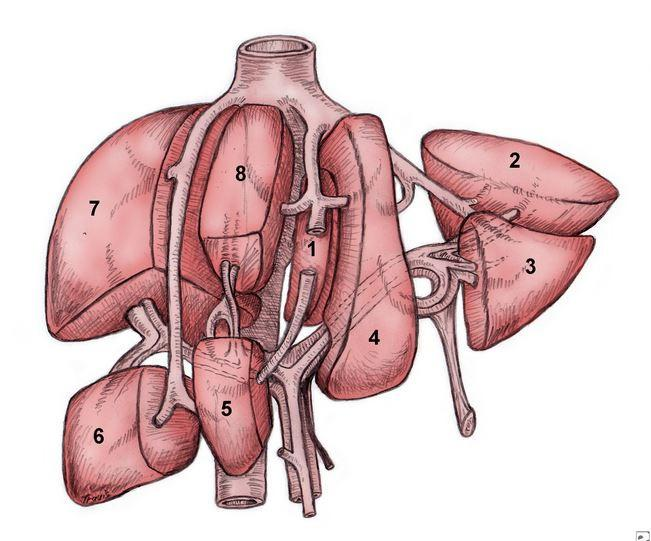
\includegraphics[width=0.5\textwidth]{Illustrations/segment.jpg}
\label{fig:segment} % Назва малюнку
\caption{Сегментарна будова печінки}
\end{figure}

Для оцінки стадії поширення пухлини печінки ключовим є розуміння судинної анатомії печінки її сегментарної будови  (Рис. \ref{fig:segment}). 
Анатомія ворітної вени (MPV) майже завжди представляє собою головний стовбур, який у воротах печінки поділяється на дві великі гілки: ліву ворітну вену та праву ворітну вену. Однак, буває інша, варіантна атаномія ворітної вени, яка найчастіше представлена трифуркацією воріної вени, або інші варіанти.
Анатомія печінкових вен набагато більш варіабельна \cite{pmid22813792}. Поряд із класичною анатомією, при якій три великі вени печінки: ліва (LHV), серединна (MHV) і права (RHV) печінкові вени впадають в нижню порожнисту вену (IVC), безпосередньо перед впадінням в останню ліва печінкова вена (LHV) та серединна печінкова (MHV) зливаються у спільне устя існують інші варіанти \cite{pmid22835780}. 
Для орієнтиру середнинної печінкової вени використовують ложе жовчного міхура. Додаткові праві задні нижні печінкові вени не використовують у якості орієнтирів для стадіювання по PRETEXT (Таб. \ref{table:PRETEXTTable}).

\begin{table}[]
\caption{Cтадіювання гепатобластом по PRETEXT.}
\resizebox{\textwidth}{!}{%
\begin{tabular}{|p{0.2\linewidth}|p{0.7\linewidth}|}
\hline
\textbf{PRETEXT} & \multicolumn{1}{c|}{\textbf{Визначення}}                              \\ \hline
\textit{I}       & пухлина в межах 1 секції печінки, 3 суміжні секції вільні від пухлини \\ \hline
\textit{II}      & 1 або 2 секції залучені, 2 суміжні секції вільні від пухлини          \\ \hline
\textit{III}     & 2 або 3 секції залучені, 1 суміжна секція вільна від пухлини          \\ \hline
\textit{IV}      & 4 секції печінки охоплені пухлиною, немає вільної суміжної секції     \\ \hline
\end{tabular}%
}
\label{table:PRETEXTTable}
\end{table}

\begin{figure}[h]
\centering
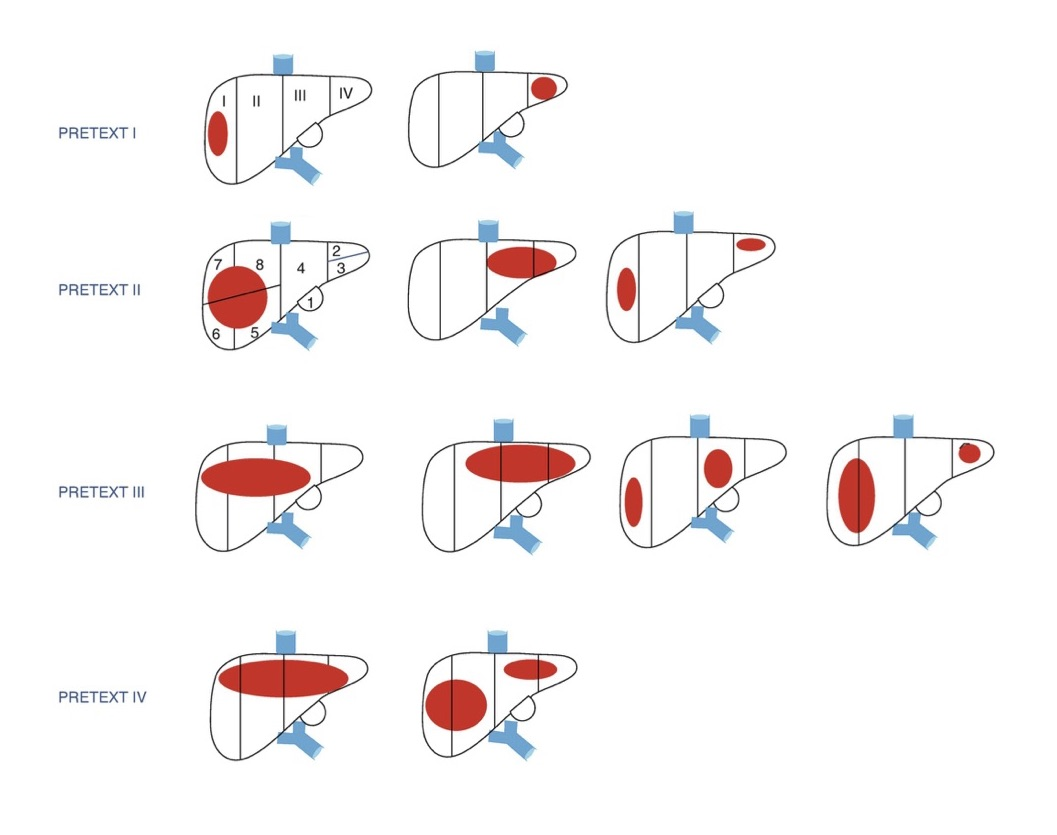
\includegraphics[width=0.9\textwidth]{Illustrations/pretexmal.jpg}
\label{fig:pretexmal} % Назва малюнку
\caption{Cтадіювання гепатобластом по PRETEXT}
\end{figure}

\subsubsection{PRETEXT I}
При цій стадії пухлина знаходиться виключно в правій задній секції печінки (сегменти 6 та/або 7)  або в лівій латеральній секції печінки (сегменти 2 та/або 3) і майже завжди резектабельна. Дуже малі пухлини найчастіше діагностується при скринінгу або як акцидентальна знахідка. Але частіше виявляються пухлини більших розмірів. 
\subsubsection{PRETEXT II}
PRETEXT II  пухлини майже завжди є однофокальними і обмежені правою або лівою долями печінки. Спочатку не було окремо класифіковано пухлини, що розміщуються лише в хвостаті долі (сегмент 1). Наразі пухлини локалізація пухлини в сегменті 1 додатково класифікується як С1.
\subsubsection{PRETEXT III}
Найважливішим завданням цієї класифікації є відрізнити PRETEXT III від PRETEXT IV. Це зробити легше для пухлин, які розташовані справа і відокремлені від лівої латеральної секції умбілікальною фісурою та ворітною веною. Коли пухлина локалізована ліворуч, основним анатомічним орієнтиром є права печінкова вена, яку часто важче ідентифікувати і яку слід відрізняти від допоміжних вен, що впадають у нижню порожнисту вену (IVC).
\subsubsection{PRETEXT IV}
При даному враженні пухлини охоплюють усі чотири відділи печінки, і тому, за надзвичайно рідкісними винятками, неможливо виконати видалення пухлини без трансплантації печінки. Результати досліджень SIOPEL свідчать про те, що багато дітей з великою однофокальною гепатопластомою PRETEXT IV перенесли трисекціонектомію після передопераційної хіміотерапії. Також є дані про мультифокальні гепатобластоми з PRETEXT IV, які також успішно лікуються без трансплантації. Незважаючи на ці спостереження, усіх пацієнтів з PRETEXT IV слід направляти на оцінку до центру трансплантації.

% Please add the following required packages to your document preamble:
% \usepackage{graphicx}
% \usepackage[table,xcdraw]{xcolor}
% If you use beamer only pass "xcolor=table" option, i.e. \documentclass[xcolor=table]{beamer}
\begin{table}[]
\caption{Субкласифікація PRETEXT}
\label{table:subPRETEXT}
\centering
\resizebox{\textwidth}{!}{%
\begin{tabular}{|
>{\columncolor[HTML]{FFFFFF}}c |
>{\columncolor[HTML]{FFFFFF}}l |}
\hline
\textbf{Субкласифікація} & \textbf{Визначення}                                                   \\ \hline
\textit{M}               & Віддалені метастази (легені)                                    \\ \hline
\textit{P}               & Інвазія пухлини в праву і ліву гілки портальної вени або в біфуркацію \\ \hline
\textit{V}               & Інвазія пухлини у нижню порожнисту вену або в печінкові вени          \\ \hline
\textit{F}               & Мультифокальна пухлина                                                \\ \hline
C                        & Пухлина каудальної долі                                               \\ \hline
E                        & Суміжна позапечінкова пухлина                                         \\ \hline
R                        & Спонтанний розрив пухлини                                             \\ \hline
\end{tabular}%
}
\end{table}



\subsubsection{Мультифокальна пухлина (F)}
При діагностиці гепатобластом важливою є також диференціація між уніфокальним та мультифокальним ростом пухлин \cite{pmid24132546}. Наявність більш ніж одного внутрішньопечінкового вузлика, незалежно від розміру або групи PRETEXT, класифікується як F1, а одиничне ураження як F0 \ref{table:subPRETEXT}.
\subsubsection{Судинні інвазії (P, V)}
При гепатобластомі так як і при гепатоцелюлярній карциномі досить часто спостерігається інвазія пухлин як в ворітну вену так і в печінкові вени та/або нижню порожнисту вену. Згідно PRETEXT 2005 року поняття інвазія визначено досить чітко окреслено: перший тип - це інвазія в просвіт вени і другий - це повне проростання вени, з обструкцією її просвіту або без нього. Припускається, що вена інвазована, якщо в проекції її розташування не візуалізується жодна судина у відповідній фазі контрастуванян. Хоча обидва варіанти є поганими прогностичними факторами. 
Інвазія або лівої ворітної вени LPV, або правої ворітної вени RPV, або однієї з їх основних гілок класифікується як P1. При інвазії обох гілок ворітної вени та/або MPV пацієнт класифікується як Р2.
Залучення однієї або двох печінкових вен або їх основних притоків класифікується як V1 або V2, відповідно. Термін V3 використовується, коли є ураження всіх трьох печінкових вен та/або IVC. Компресія IVC дуже часто спостерігається у дітей з великими пухлинами, часто супроводжується збільшенням напівнепарної вени.
У кожному випадку втягнення вен (на відміну від огортання) позначається суфіксом –a.
\subsubsection{Позапечінкове поширення пухлини (E, H)}
Система PRETEXT класифікує пряме поширення пухлини з печінки та перитонеальне поширення пухлини як E1, E1a, E2 або E2a \cite{pmid23217875}. Крім того, при обстеженні також встановлюється наявність (H1) або відсутність (H0) розриву пухлини. Хоча немає жодних доказів того, що E1, E2 або H1 є несприятливим прогнозом.

Первинна пухлина печінки може проростати в черевну стінку, діафрагму або сусідні органи, такі як підшлункова залоза або товста кишка \cite{pmid23331862}. Пряме проростання пухлини класифікується як Е1. Проростання лише в жовчний міхура не слід розглядати як E1.
Канцероматоз очеревини у вигляді окремих пухлинних вузликів часто можна виявити за допомогою КТ або МРТ особливо у пацієнтів з асцитом (рис. 8.13; \cite{pmid23831416}. Це поширення класифікується як E2, незалежно від розміру ураження.

Невідомо, чи наявність асциту є незалежним фактором ризику у дітей з первинними пухлинами печінки. Для полегшення подальшого аналізу даних до класифікації додається суфікс –a (тобто E0a, E1a або E2a), коли присутній асцит.

Розрив пухлини класифікується як Н1. За звичай це проявляється  клінічниими, лабораторними та візуалізаційними методами досліджень. Наприклад, поява раптового болю у животі, можливо, після травми, гіпотонія або зниження рівня гематокриту та поява ехогенної рідини в черевній порожнині на УЗД, або аспірація крові при пункції. Розрив пухлини не рідкість для паціїнтів з гепатобластомою \cite{pmid24132546}, і може знадобитися термінова операція або емболізація. Локалізовані (наприклад, субкапсульні) крововиливи та кровотечі, пов’язані з біопсією, не класифікуються як H1.
\subsubsection{Метастатична хвороба (M, N)}
Як і у дорослих, пухлини гематогенні метастази класифікуються як M1. При гепатобластомі майже всі метастази при діагностиці виявляються в легенях (M1p), але при ураженні інших пухлин, наприклад гепатоцелюлярній карциномі іноді зустрічається в скелет (M1s), центральній нервовій системі (M1c), кістковому мозку (M1m) або інших ділянках (M1x). Підтверджувати метастаз біопсією при наявності переконливих даних не потрібно.  

Хоча мультидетекторна технологія КТ зараз широко доступна, якісна візуалізація всієї поверхні легенів часом неможлива з різних причин, незважаючи на анестезію або седацію пацієнтів. Навіть при ідеальній візуалізації діагностика легеневих метастазів у дітей складна \cite{pmid24362406}. Різні доброякісні ураження можуть імітувати поодинокі або множинні метастази. Найпоширеніші з них - гранульоми, які можна спостерігати після бактеріальних, грибкових або вірусних інфекцій (наприклад, туберкульозу, гістоплазмозу та вітряної віспи). Гамартоми та внутрішньолегеневі лімфатичні вузли також можуть імітувати метастази.

Система PRETEXT застосовує прагматичний підхід до вирішення цієї проблеми. Замість того, щоб наполягати на біопсії у всіх пацієнтів із ураженнями легень, сумісними з метастазами, він класифікує їх як M1p і залишає рішення про стратифікацію ризику (наприклад, на основі розміру та/або кількості уражень) для індивідуального лікування. 

Метастази в лімфатичні вузли є рідкісними при гепатобластомі \cite{pmid24734315}, і навіть коли вони є, на даний момент не до кінця зрозуміло чи вони є значущим прогностичним фактором \cite{pmid24757164}. Також вони можуть бути збільшені у наслідок запального процесу. З цих причин по системі PRETEXT необхідно підтвердження біопсії. У перспективі виявлення злоякісних вузлив за допомогою позитронно-емісійна томографія або дифузійно-зваженого МРТ. В даний час найкращим підходом може бути біопсія дуже великих вузлів (> 15 мм у ширину) у дітей з гепатобластомою \cite{pmid24759227}. 

Метастази в черевні лімфатичні вузли кодуються як N1, а віддалені вузлові метастази як N2.
\subsection{Післяопераційна класифікація Children’s Oncology Group }

Згідно цієї класифікації при I стадії у пацієнта відсутні метастази і пухлина повністю резектована. При ІІ стадії відсутні метастази, немає мікроскопічної інвазії після резекції пухлини або розриву пухлини (включаючи розлив пухлини під час операції). При ІІІ стадії немає віддалених метастазів, пухлини нерезектабельні або резектовані з грубими залишковими вогнищами або є метастази у лімфатичні вузли. При ІV стадії є віддалені метастази, не залежно від місцевого поширення пухлини \cite{pmid24852330}.

% Please add the following required packages to your document preamble:
% \usepackage{graphicx}
% \usepackage[table,xcdraw]{xcolor}
% If you use beamer only pass "xcolor=table" option, i.e. \documentclass[xcolor=table]{beamer}

\begin{table}[]
\small
\caption{Післяопераційна класифікація Children’s Oncology Group\cite{pmid24852330}}
\label{table:subPRETEXT}

\centering

\normalsize
\begin{tabular}{|p{0.15\linewidth} | p{0.6\linewidth}|}
\hline
\textbf{Стадія}                                    & \textbf{Визначення}                                                                     \\ \hline
{\color[HTML]{202124} \textit{\textbf{Стадія I}}}  & {\color[HTML]{202124} Відсутні метастатичні захворювання, пухлина повністю резектована} \\ \hline
{\color[HTML]{202124} \textit{\textbf{Стадія IІ}}} &
  {\color[HTML]{202124} Відсутність метастатичного захворювання, 
  мікроскопічного залишкового захворювання після резекції пухлини або розриву пухлини 
  (включаючи розлив пухлини під час операції)} \\ \hline
{\color[HTML]{202124} \textit{\textbf{Стадія IІI}}} &
  {\color[HTML]{202124} Немає віддалених метастазів, 
  пухлини нерезектабельної або 
  резекованої з грубими залишковими захворюваннями 
  або метастазів у лімфатичні вузли} \\ \hline
{\color[HTML]{202124} \textit{\textbf{Стадія IV}}} & {\color[HTML]{202124} Далекі метастази, незалежно від місцевого поширення пухлини}      \\ \hline
\end{tabular}%

\end{table}


% Please add the following required packages to your document preamble:
% \usepackage{graphicx}
% \usepackage[table,xcdraw]{xcolor}
% If you use beamer only pass "xcolor=table" option, i.e. \documentclass[xcolor=table]{beamer}
\begin{table}[]
\centering
\caption{Групи ризику гепатобластом по системі CHICS (Children’s Hepatic Tumors International Collaboration`s Stratification)}
\label{tab:risk}
\resizebox{\textwidth}{!}{%
\begin{tabular}{{|p{0.15\linewidth} | 
                  p{0.15\linewidth}|
                  p{0.15\linewidth}|
                  p{0.15\linewidth}|
                  p{0.15\linewidth}|
                  }}
\hline
\textbf{Групи ризику} &
  {\color[HTML]{231F20} \textbf{LR (low risk) – група низького ризику}} &
  {\color[HTML]{231F20} \textbf{IR (intermediate risk) – група среднього ризику}} &
  {\color[HTML]{231F20} \textbf{HR (high risk) – група високого ризику}} &
  {\color[HTML]{231F20} \textbf{VHR (very high risk) – група вкрай високого ризику}} \\ \hline
{\color[HTML]{231F20} \textit{\textbf{Метастази}}} &
  {\color[HTML]{231F20} \textbf{М(-)}} &
  {\color[HTML]{231F20} \textbf{М(-)}} &
  {\color[HTML]{231F20} \textbf{М(-)}} &
  {\color[HTML]{231F20} \textbf{М(+)}} \\ \hline
{\color[HTML]{231F20} \textit{\textbf{I}}} &
  {\color[HTML]{231F20} VPERF—, (будь-який AFP, будь-який вік)} &
  {\color[HTML]{231F20} -} &
  {\color[HTML]{231F20} VPERF+ , та вік \textless{}8 лет (будь-який AFP)} &
  {\color[HTML]{231F20} VPERF+, і вік ≥8 років} \\ \hline
{\color[HTML]{231F20} \textit{\textbf{II}}} &
  {\color[HTML]{231F20} VPERF—, вік \textless 3 років та AFP \textgreater{}1,000 ng/mL} &
  {\color[HTML]{231F20} VPERF—, вік \textless 3років, та AFP 100-1,000 ng/mL} &
  {\color[HTML]{231F20} Вік 3-7 роки, та/або VPERF +} &
  {\color[HTML]{231F20} AFP \textless{}100 ng/mL, та/або вік ≥8 років} \\ \hline
{\color[HTML]{231F20} \textit{\textbf{III}}} &
  {\color[HTML]{231F20} -} &
  {\color[HTML]{231F20} VPERF—, та вік \textless 3років, та AFP \textgreater{}1,000 ng/mL} &
  {\color[HTML]{231F20} Вік 3-7 роки, та/або VPERF+, та/або AFP 100-1,000 ng/mL} &
  {\color[HTML]{231F20} AFP \textless{}100 ng/mL, та/або вік ≥8 років} \\ \hline
{\color[HTML]{231F20} \textbf{IV}} &
  {\color[HTML]{231F20} -} &
  {\color[HTML]{231F20} -} &
  {\color[HTML]{231F20} AFP \textgreater{}100 ng/mL} &
  {\color[HTML]{231F20} AFP \textless{}100 ng/mL, та/або вік ≥8 років} \\ \hline
\end{tabular}%
}
\end{table}


\begin{figure}[h]
\centering
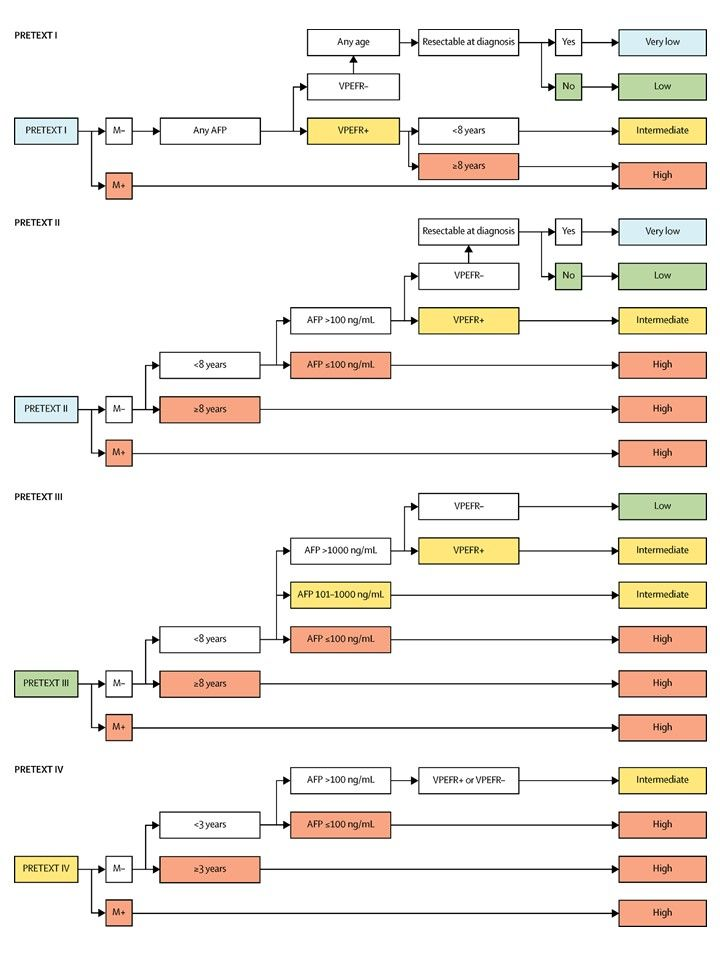
\includegraphics[width=0.9\textwidth]{Illustrations/risk.jpg}
\label{fig:risk} % Назва малюнку
\caption{Групи ризику гепатобластом по системі CHICS (Children’s Hepatic Tumors International Collaboration`s Stratification)\cite{pmid24757164}}
\end{figure}